\documentclass[11pt,oneside,a4paper,notitlepage]{book}

\usepackage[utf8]{inputenc}
\usepackage[ngerman]{babel}
\usepackage[margin=1.25cm]{geometry}

%kommentare, zitate, quellcode
\usepackage{verbatim}
%\fontfamily{sfdefault}
\renewcommand{\familydefault}{\sfdefault}
%
\usepackage{graphicx}
%fuer tabellen
\usepackage{tabularx}
\usepackage{tabulary}
%referenzen und links
\usepackage{hyperref}
\hypersetup{
colorlinks=false,
hidelinks=true
}
%

%
\newcommand{\brand}{TAARs }
%
\newcommand{\anm}[1]{\begin{comment} #1 \end{comment} }
%
% - - - - - - - - - - - - - - - - - - 
%
\begin{document}


\begin{center}
\Large{EIS WS1516 - Meilenstein 2}\\[3mm]
\normalsize{Verteiltes Training einer automatisierten Dokumentenattributierung}\\[3mm]
\normalsize{Tim Howe}
\end{center}

\brand - Verteilte Group- Middleware zum Training einer automatisierten Attributierung von Rechnungen


\tableofcontents


\newpage

\chapter{Systembeschreibung}
Ein allgemeine Beschreibung der wichtigsten Eigenschaften des \brand , detaillierte Beschreibungen folgen in den 
zugehörigen Kapiteln

%
\section{Komponenten}

\paragraph*{Verwaltungsserver}

\begin{enumerate}
\item importiert Rohdaten, erzeugen des Geschäftsobjekts
\item prüft Rohdaten auf Vollständigkeit, vorhandene Regeln, falls eine vollständige Regel 
\begin{enumerate}
\item vorliegt: Übergabe des Geschäftsobjekts an den Regel-Server
\item nicht vorliegt: Übergabe des Geschäftsobjekt an einen Verwaltungsclient
\end{enumerate}
\item erhält vervollständigte Geschäftsobjekte von Verwaltungs- und Fachclient
\item gibt Informationen zum Systemzustand an Steuerungsclient
\end{enumerate}

%
\paragraph*{Verwaltungsclient}

\begin{enumerate}
\item Windows Desktop Client
\item erhält unvollständige Geschäftsobjekte vom Verwaltungsserver
\item vervollständigt diese Geschäftsobjekte
\item sendet vollständige Geschäftsobjekte an Verwaltungsserver
\item sendet unvollständige Geschäftsobjekte an Fachclient
\item verwaltet angelegte Regeln
\end{enumerate}

%
\paragraph*{Fachclient}
\begin{enumerate}
\item Windows Desktop Client
\item funktionale Untermenge des Verwaltungsclients
\item erhält unvollständige Geschäftsobjekte vom Verwaltungslcient
\item sendet vollständige Geschäftsobjekte an Verwaltungsserver
\end{enumerate}

%
\paragraph*{Steuerungsclient}

\begin{itemize}
\item erhält Informatinen zum Systemzustand vom Verwaltungssserver
\item übergibt Priorisierungskommandos an Verwaltungsserver
\end{itemize}

%
\paragraph*{Regel-Server}
\begin{enumerate}
\item erhält Geschäftsobjekt von Veraltungsserver
\item berechnet die Anwendung der Regel auf das Geschäftsobjekt
\item exportiert das Ergebnis
\end{enumerate}


%
\section{Nutzerrollen}



\section{Geschäftsobjekt}
Das verarbeitete Geschäftsobjekt besteht aus den Rohdaten einer Rechnung, den zugehörigen Metadaten und einer zugewiesenen Regel für
dieses Geschäftsobjekt.
\chapter{Zielhierarchie}
\label{cha:zielhierarchie}

\begin{comment}
Eine Zielhierarchie lässt sich in drei Ebenen strukturieren.
+ strategische Ziele sind Ziele, die auf langfristige Sicht erreicht werden sollen. 
	Strategische Ziele beantworten die Frage "Was soll erreicht werden?"
+ taktische Ziele sind Ziele, die auf mittelfristige Sicht erreicht werden sollen.
	Taktische Ziele beantworten die Frage "Wie soll es erreicht werden?"
+ operative Ziele sind Ziele, die auf kurzfristige Sicht erreicht werden sollen.
	Operative Ziele beantworten die Frage "durch welche Aktivitäten soll es erreicht werden?" 
Die Zielpriorisierung sollte sich durch die verwendeten Verben (muss,soll,kann) ausdrücken. 
\end{comment}


\section{Strategisch}
\label{sec:zielhierarchie-strategisch}

\begin{enumerate}
\item Objektbereich:\\
Es muss ein Komplexitätsgrad erreicht werden der fachlich relevant und technologisch, im Rahmen des Projekts, beherrschbar ist
\item Anwendungsdomäne:\\
Es soll ein Anwendungskontext mit möglichst hoher wirtschaftlicher Relevanz gefunden werden
\item Technologisch:\\
Es sollen möglichst viele im beruflichen Kontext relevanten Erfahrungen... , siehe \nameref{}
\item Nutzung:\\
Anwender sollen vom Ballast repetiver Aufgaben befreit werden
\end{enumerate}


%
\section{Taktisch}
\label{sec:zielhierarchie-taktisch}

\begin{enumerate}
\item Anwendungskontext \& Objektbereich:\\
Es muss eine qualifizierte Entscheidungsgrundlage geschaffen werden
\item Technologisch:\\
Implementierungrelevante Entscheidungen sollen gegen den beruflichen Kontext bewertet werden
\item Nutzung:\\
Es soll Automatisierungspotential identifiziert werden
\item ...
\end{enumerate}


%
\section{Operational}
\label{sec:zielhierarchie-operational}

\begin{enumerate}
%
\item Anwendungskontext \& Objektbereich:\\
Es muss eine Analyse und Bewertung der in den Anwendungsdomänen genutzen Objekte, dh. Dokumentenklassen, durchgeführt werden
\item Technologisch:\\
Begründen wenn vom definierten Standard \href{sec:entscheidungen} abgewichen wird
\item Nutzung:\\
\begin{enumerate}
\item deskriptive Aufgabenanalyse
\item Automatisierungspotential identifizieren
\item präskriptive Aufgabenanalyse, inkl P2
\end{enumerate}
\item ...
\end{enumerate}




\chapter{Marktrecherche}

\begin{comment}
Die Marktrecherche, auch related works genannt, beinhaltet die Recherche nach konkurrierenden Systemen, die teilweise oder vollständig die Funktionalitäten aufweisen wie sie für das zu entwickelte System geplant sind. Dabei sollte man Vor- und Nachteile gegenüber dem zu entwickelten System herausstellen. 
\end{comment}

Der Markt wird im allgemeinen von Entwicklern einzelner Komponenten und Systemhäusern bestimmt die Fremdkomponenten ggf mit Eigenentwicklungen kombinieren und so individuelle Lösungspakete schnüren.\\
Die Komponenten lassen sich grob in die folgenden Bereiche enteilen:
\begin{itemize}
\item OCR: Scannen, Klassifizieren
\item Workflow
\item betriebliche Anwendungssysteme: Buchhaltung, Archivierung
\end{itemize}
\noindent
Zudem sind sogenannte OEM Versionen \href{}{glossar} durchaus gängige Praxis wodurch eine Einsicht erschwert wird.\\
Um dennoch einen Eindruck in die Marktsituation zu gewinnen hilft eine Betrachtung der og Bereiche in der funktional übergeordneten Ebene der DMS -Systeme und deren Eigenschaften. Es werden Ansätze zweier Anbieter exemplarisch beschrieben und eine Einordnung zwischen diesen Lösungen und \brand mittels einer Featurematrix ermöglicht.


\section{Codia DMS }
%
% http://www.codia.de/codia/files/dms_in_hochschulenv1.pdf
%
% http://www.codia.de/codia/d.3ecm--die-basis.php
Codia DMS bietet auf Basis des d3.ecm von d.velop spezialisierte Lösungen im eGovernment Umfeld für öffentliche Verwaltung und Hochschulen mit den Themen Scannen & Klassifizierung, Rechungs- und Eingangspostverarbeitung, eAkte und Archivierung.


\section{InPunkto}
% http://www.inpuncto.com/de/sap-ecm-loesungen/prozessoptimierung-sap-workflow/elektronische-rechnungsbearbeitung/automatisierter-rechnungseingang/
InPunkto spezialisert auf Dokumenten Dienstleistungen im SAP Umfeld mit den Themen Automatische Erfassung \& Verarbeitung, Workflow, 
eAkte und Archivierung.


\section{Übersicht}
%http://www.codia.de/codia/workflow.php
%http://www.codia.de/codia/eingangsrechnungsverarbeitung.php
%


\begin{tabulary}{\textwidth}{LLLL}
Thema & Codia & InPunkto & \brand \\
Automatisierte Klassifizierung & J & J & N \\
Attributierung & & &\\
semantisch & J & kA & N\\
fachlich & J & J & J \\
Automatisierte Attributierung & N & N & J \\
Steuerung & lastabhängige Aufgabenverteilung\newline über Workflowsystem & kA & Priorisierung\\
(Rechnungs) Workflow & d3ecm & SAP Workflow & freie Wahl \\
Export & d3.ecm & SAP & Rohexport als xml\\
\end{tabulary}


\chapter{Domänenrecherche}
\label{cha:domaene}

\begin{comment}
Die Domänenrecherche zeigt auf in welcher Domäne das System zukünftig eingesetzt werden soll. Dabei soll recherchiert werden welche wichtigen Konzepte der Anwendungsdomäne eine Rolle bei der Gestaltung des Systems spielen. Es werden zudem sämtliche Informationen, Vorgänge, Metaphern und Paradigmen aus der Domäne recherchiert, in dem sich das zu entwickelnde System befindet. Die Domänenrecherche bildet die Basis für die Entwicklung eines Nutzungsproblems und der nachfolgenden Konzeption des gesamten Systems. 
\end{comment}

Im folgenden werden die wichtigsten Themen der Anwendungsdomäne beschrieben und einer ersten Bewertung
hinsichtlich projektrelevanter Eigenschaften unterzogen.



\section{Allgemeine Verarbeitungprozess}
\label{sec:domaene-prozess}
% quellen: 
% 13.10: http://www.wi.fh-flensburg.de/fileadmin/dozenten/Riggert/bildmaterial/Dokumentenmanagement/2-Capture-Klassifikation___Extraktion.pdf
% 13.10: 
%

Beispielhaft die wichtigsten funktionalen Komponenten des Dokumentenverabreitungsprozesses beschrieben, wichtig bleibt anzumerken
das in konkreten Implementierungen die Funktionalitäten verschwimmen und keine klare Trennung wie hier beschrieben vorherrscht(?). 
%
% wichtig für Architektur > Marktrecherche(?)
%

\begin{enumerate}
\item Extraktion:\\
Manuelles oder mittels OCR automatisiertes auslesen von Informationen aus einer Dokumentendatei oder einer zugehörigen Bitmapdatei.
\begin{enumerate}
\item optional Nacherfassung:\\
Kontrolle der OCR Ergebnisse und ggf Korrektur bei unzureichender Extraktionsqualität
\end{enumerate}
\item Klassifizierung:\\
Beschreibt die Einordnung in eine klar abgegrenzte Menge von Dokumenttypen wie zb. Formulare, Rechnungen, Lieferscheine, 
Bewerbungen.
\item Attributierung:\\
Beschreibt den Prozess der Zuordnung von organisations- oder fachspezifischen Attributen zu einem Dokument zur weiteren
Verarbeitung innerhalb der Organisation. Die können zum Beispiel Buchungskonten, Kostenstellen, Projektnummern oder Anprechpartner   sein.
\item Export \& weitere Verarbeitung:\\
Übergabe der klassifizierten und attributierten Dokumente an einem betriebliches Anwendungssystem zur Buchung, Kontierung oder Archivierung.
\end{enumerate}
\noindent

%
\section{Der Begriff der Attributierung}
In der Praxis wird der Begriff der Attributierung für zweierlei Aspekte verwendet:\\
%, häufig unscharf definiert 
\begin{enumerate}
\item semantische(?) Attributierung:\\
Extrahierung und Zuordnung von Metainformationen zu einem Dokument welche sich auf das Dokument, bzw die Dokumentendatei als Repräsentation des Dokuments, selbst beziehen. Dies können zb Schlagworte, Speicherort ... sein.
\item fachliche Attributierung:\\
Die fachliche Attributierung ist ein Teil des Arbeitsprozesses bei welchem dem Dokument Attribute zugeordnet werden die 
Diese Attribute können zb kaufmännischer, steuerlicher oder juritischer Natur sein.
\end{enumerate}
\noindent
Für dieses Projekt wird der Begriff im Sinne der fachlichen Attributierung verwendet.

\section{Strukturierungsgrad}
\label{sec:domaene-struturierungsgrad}

Der Strukturierungsgrad eines Dokuments wird beschrieben durch das Ausmaß an Sicherheit mit der ein Wert eines Dokumentenattributs
an einer Position im Dokument auftritt und welcher Wertebereich in diesem abgebildet wird.
	
\begin{enumerate}
\item unstrukturiert: gar keine bis geringe Positionssicherheit mit überwiegend undefiniertem Wertebereich, zb. Bewerbungsschreiben
\item semi-strukturiert: gute Positionssicherheit mit überwiegend definiertem Wertebereich, zb. Rechnungen, Lieferscheine
\item strukturiert: absolute Positionssicherheit mit klar definiertem Wertebereich, zb. genormte betriebliche oder behördliche Formulare
\end{enumerate}
\noindent
%Je höher der Strukturierungsgrad eines Dokumenttyps desto spezialisiertier besser eignet sich dieser für eine automatisierte Verarbeitung.
Mit dem Strukturierungsgrad steigt die semantische Spezialisierung sowie das Automatisierungspotential für diesen Dokumenttyp.

%
\newpage

\section{Anwendungsfelder}
\label{sec:domaene-anwendungsfelder}

\begin{table}[ht]
\caption{Automatisierte Dokumentenverarbeitung}\\
  \begin{tabulary}{\textwidth}{LLLL}
Domäne 		& Primäre Dokumenttypen 	& Strukturierungsgrad 	& wirtschaftliche Relevanz  \\ 
\hline \\
Buchhaltung	& Rechnungen				& 2 						& ++\\ 
\hline
Verwaltung	& Formulare 				& 3 						& + \\
 \hline
Personal 	& Bewerbungen 			& 1-2 					& o \\ 
\hline
Kanzleien 	& Schriftverkehr			& 1						& + \\ 
\hline
Logistik 	& Lieferscheine 			& 2 						& + \\
%\hline Produktion	&	...					& 2						& + \\
\hline
Privat 		& Rechnungen\newline 
			Versicherungen\newline
			Formulare				& 2\newline
									  1\newline
									  3 						& -\newline
									  							Services für Privatanwender\newline nicht etabliert 
  \end{tabulary} 
\end{table}
\noindent


\section{Nutzungsmerkmale}

Eine erste kurze Betrachtung der antizipierten Nutzungsmerkmale welche Entscheidungen zu Anwendungsdomäne (ref), Objektbereich (ref)
und ... unterstützen soll.

\begin{table}[ht]
\caption{Nutzungsmerkmale}\\
\begin{tabulary}{\textwidth}{LLL}
Domäne		& Arbeitsumgebung & Arbitsgerät(?) & Organisationsrolle\\
\hline \\
Buchhaltung	& Büro & Desktop PC & Bürokfm Fachkraft \\
\hline
Verwaltung	& Büro & Desktop PC & Bürokfm oder Verwaltungs- Fachkraft \\
\hline
Personal 	& Büro & Desktop PC & Personaldienstleistungskfm Fachkraft\\ 
\hline
Kanzleien 	& Büro & Desktop PC & Bürokfm Fachkraft\\ 
\hline
Logistik 	& Büro\newline ggf Mobil, in größeren Betrieben & Desktop PC\newline ggf Tablet & Bürokfm Fachkraft, Lagerist\\
%\hline Produktion	& Werkhalle	& \\
\hline
Privat 		& Zuhause\newline Mobil & Desktop PC\newline Tablet, Smartphone & Privat, Organisieren von Post(?) \\ 
\end{tabulary}
\end{table}
\noindent
%
\newpage




\chapter{Alleinstellungsmerkmale}

\begin{comment}
Alleinstellungsmerkmale sind jene Merkmale oder Funktionalitäten, die das System auszeichnen und sich somit gegenüber anderen Systemen abhebt. Die Alleinstellungsmerkmale lassen sich oft aus der Marktrecherche ableiten bzw. daraus argumentieren. 
\end{comment}


Die Markt- und Domänenanalyse offenbart (hoffentlich!!!) eine Marktlücke für Firmen mit
\begin{enumerate}
\item mit einem bestehenden Extrahierungsprozess und optionalem Nacherfassungsprozess
\item mit einem bestehenden Buchungs- , Kontierung- oder Archivssystem
\item Workflow
\begin{enumerate}
\item mit bestehendem Workflowsystem oder
\item ohne Bedarf für ein vollintegratives Workflowsystem
\end{enumerate}
\item mit Bedarf für eine Automatisierung
\end{enumerate}


%
\paragraph{Slim Clients}


\paragraph{Automatisierte Attributierung}


%
\paragraph{freie Wahl des Workflowsystem}
Für ein Workflowsystem muessen 






\chapter{Methodischer Rahmen}

\begin{comment}
Der methodische Rahmen bezieht sich auf die Wahl des MCI Vorgehensmodells und sollte vorab definiert werden. Im methodischen Rahmen werden angemessene Methoden für jegliche Aktivitäten und Unteraktivitäten festgelegt, welche projektspezifisch (d.h. aus dem Problemraum heraus) definiert und begründet sind. Mögliche Iterationen sollten berücksichtigt werden.
\end{comment}
\chapter{Kommunikationsmodel}

\begin{comment}
Im Kommunikationsmodell muss ersichtlich sein, welche Informationen zwischen Nutzern in verschiedenen Rollen über das System ausgetauscht werden sollen. Dabei kann es auch wichtig sein die Reihenfolge der Kommunikationsvorgänge zu spezifizieren. 
\end{comment}

\section{Akteure}

\subsection*{Verwaltungsdienst}
\begin{itemize}
\item übergibt Rohdaten und Regeln an Regel-Engine
\item gibt Informationen zum Systemzustand an Steuerungsclient
\item erhält Priorisierungsinformation von Steuerungsclient
\item übergibt priorisiertes Geschäftsobjekt an Verwaltungsclient
\end{itemize}

\subsection*{Steuerungsclient}
\begin{itemize}
\item erhält Information vom Verwaltsdienst zum Systemzustand %@todo verschieben welche Absender aktuell sind wie lange im System
\item teilt Verwaltungsdienst die Priorisierung mit%@todo an andre stelle: nach Eingangsdatum (FIFO), Absender, ggf Anzahl/Absender
\end{itemize}

\subsection*{Verwaltungsclient}
\begin{itemize}
\item erhält aktuell priorisierte Geschäftsobjekte vom Verwaltungsdienst
\item gibt vollständiges Geschäftsobjekt an Verwaltungsdienst zurück
\item gibt unvollständiges Geschäftsobjekt an Fachclient (über Verwaltungsdienst)
\end{itemize}

\subsection*{Fachclient}
\begin{itemize}
\item erhält unvollständiges Geschäftsobjekt von Verwaltungsclient (über Verwaltungsdienst)
\item gibt vervollständigtes Geschäftsobjekt an Verwaltungsdienst zurück
\end{itemize}

\subsection*{Regel-Engine}
\begin{itemize}
\item erhält Geschäftsobjekt und Regel vom Verwaltungsdienst
\end{itemize}


\section{Kommunikationsdiagramm}

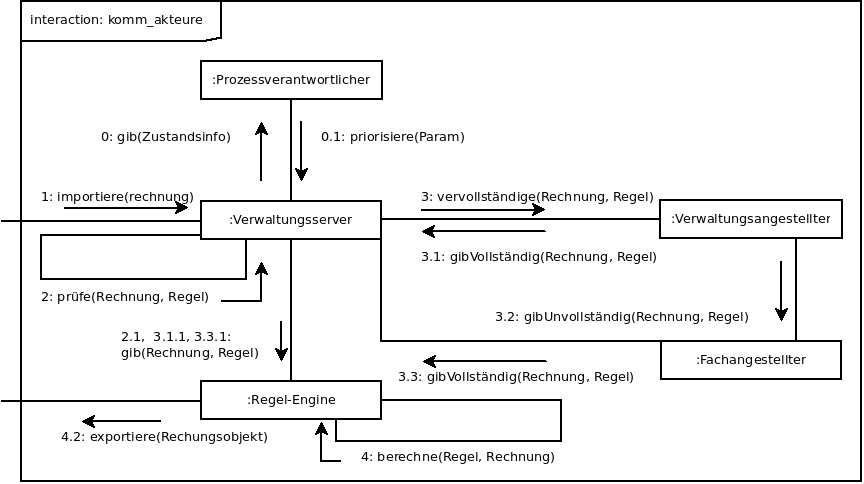
\includegraphics[width=\textwidth]{EISWS1516Howe_Kommunikation.png}
\noindent




\chapter{Risiken}

\begin{comment}
Risiken können Ereignisse sein, die den Projektverlauf auf eine bestimmte Art und Weise gefährden könnten. Relevant sind dabei projektspezifische Risiken. Es ist wichtig sie vorab zu identifizieren und entsprechende Maßnahmen zu planen, um dieses Risiko zu minimieren bzw. den Umgang zu beschreiben, falls dieses Risiko auftritt. Technische Risiken sollten mit Hilfe eines Proof of Concept minimiert werden. Dementsprechend ist es wichtig zu beschreiben wie die Risiken mit einem PoC adressiert werden. 
\end{comment}



%
\section{Architektur}


\paragraph*{Zugriffsstruktur \& Steuerung}

Es muss eine Struktur gefunden werden mit der die folgende Funktionalitäten unabhängig voneinander 
realisiert werden können:
\begin{enumerate}
\item Zugriff des Verwaltungsclients auf Geschäftsobjekte
\item Übergabe der Geschäftsobjekte von Verwaltungsclient an den Fachclient
\item Steuerung der Priorisierung der Geschäftsobjekte\\

\end{enumerate}

%zugriffs struktur der clients auf Geschäftsobjekte: Paradigma das Lose Kopplung unterstützt -- bestenfalls unabhängig von Requests durch Clients
%


\paragraph*{Steuerungsclient}

\begin{enumerate}
\item kommunikation zu steuerungskomponente im Verwaltungsdienst
\item Implementierung von interaktionsparadigmen (?)
\end{enumerate}
\item 
\end{enumerate}

%
\paragraph*{Regel-Engine}
Es muss eine Regelform entwickelt werden die die strategischen Ziele 1 + 2 erfüllt.
Definition und Speicherung des Regelobjekts sowie Anwendung der Regeln auf Geschäftsobjekte.


\begin{comment}
%
\section{Marktzugang}
\paragraph*{Direkt}
Ein Integration in einen bestehenden Prozess einer Firma könnte schwierig sein wenn Firmen dieses Projekt als zu fragmentiert ansehen und lieber Lösungen "aus einer Hand" haben wollen.
%
\paragraph*{Partner}
Beim Marktzugang über Partner wie DMS Hersteller und Systemhäuser könnte die \brand Kernfunktionalität der Attributierung nicht als Mehrwert schaffende Zusatzkomponente angesehen werden.
%
\section{Fachlich}
Firmeninterne oder gesetzliche Regeln zur Dokumentenverarbeitung könnten den Verwaltungsaufwand der einen Attrbutierungsprozess umgibt 
unvorhergesehen erhöhen.
\end{comment}


\chapter{Proof of Concepts}

\begin{comment}
Die Proof of Concepts lassen sich evtl. aus den Risiken ableiten. Für die Spezifizierung der Proof of Concepts müssen jeweils Exit- und Failkriterien beschrieben werden. D.h. es werden konkrete Bedingungen spezifiziert, die besagen in welchem Fall ein Proof of Concept als "erfolgreich" oder als "nicht erfolgreich" gilt. Falls ein Proof of Concept gescheitert ist, muss man sich im Vorfeld Alternativen/Fallbacks überlegen, die anstelle der ursprünglich angedachten Vorgehensweise herangezogen werden könnten. Die Durchführung eines Proof of Concepts muss dokumentiert werden. 
\end{comment}


\section{Architektur}


\section{technisch: mobiler Client}

\begin{itemize}
\item ruft api des verwaltungsdienstes auf
\item erhält json(?) objekt mit Informationen zum Systemzustand
\item ruft Steuerungs api mit Priorisierungsparameter auf
\end{itemize}


\section{technisch: Steuerungsaip & Dienst}
\chapter{Prozess}
%
% immer wieder prüfen of dokumentarisch wertvoll oder ob KommModel & Architektur alles bedienen 
%
Ausgehend von \textit{Domaenenrecherche \> Prozess} eine Darstellung des eines exemplarischen Verarbeitungsprozesses und 
die Intergration des zu entwickelnden \brand in diesen.

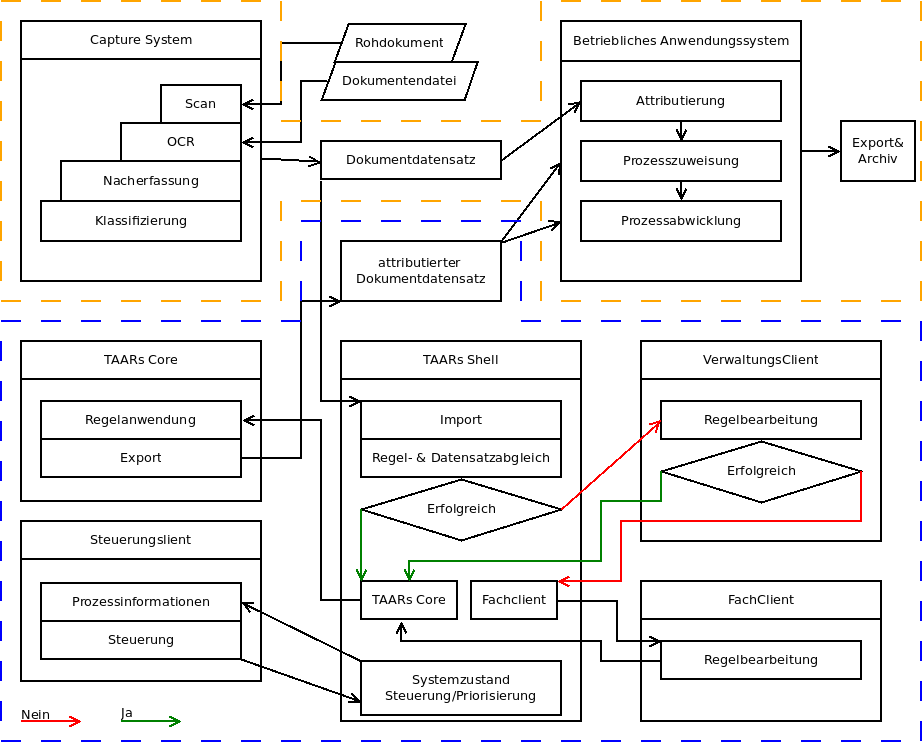
\includegraphics[width=\textwidth]{EISWS11516Howe_Prozess.png}
\noindent
\chapter{Architekturdiagramm}

\begin{comment}
Im Architekturdiagramm muss ersichtlich sein welche Softwareschichten/Softwarekomponenten es im System gibt und über welche Kommunikationsprinzipen und Protokolle diese miteinander kommunizieren. Es muss aufgezeigt werden wie die ausgetauschten Informationen repräsentiert werden. Des Weiteren spielt die Verteiltheit der Anwendungslogik eine große Rolle. 

Es muss nachvollziehbar sein inwiefern eine Verteiltheit der Anwendungslogik gegeben ist. 

Sämtliche Entscheidungen müssen begründet und abgewogen werden. Formal gesehen sollten einfache geometrische Primitive verwenden werden. (Orientierung an der Fachliteratur) 
\end{comment}


\section{Übersicht}
- bsp arch\\
- arch mit ASys\\
- 

\section{Verwaltungsdienst}

\section{Clients}

\subsection{Verwaltung}
\subsection{Fachclient}

\section{Steuerungsclient}


\section{Regel-Engine}





\chapter{Projektplan}

\begin{comment}
Ein Projektplan wird innerhalb der Projektlaufzeit laufend fortgeführt. Sämtliche Projektaktivitäten werden chronologisch aufgelistet und in Unteraktivitäten gegliedert (mind. drei Gliederungsebenen). Dabei soll zu den Aktivitäten die geplante Zeit gegenüber der tatsächlich verbrauchten Zeit in Stunden angegeben werden. Zudem sollte eine Zuweisung zu den Teammitgliedern erfolgen.
\end{comment}

Der Projektplan wird zunächst \href{run:../EISWS1516_Howe_Projektplan.ods}{hier} geführt.
\chapter{Projektbegründungen}

\begin{comment}
Die Projektbegründungen sind jene Begründungen, die Bezug nehmen auf jegliche Entscheidungen, die im Projekt getroffen werden. Es sind somit projektspezifische Begründungen. Darin sollten Alternativen abgewägt werden und Inhalte auf den Punkt gebracht werden, sodass "Totes Wissen" eliminiert wird. Ein roter Faden sollte ersichtlich sein. Als Referenz dienen jeweilige Artefakte, die in dem Projekt entwickelt worden sind und demnach begründet werden müssen. 
\end{comment}


\section{Implementierung}
Die Entscheidung der Implementierungsumgebung wird aus den strategischen Zielen \ref{sec:zielhierarchie-strategisch}
sowie Punkt 3 der Kursziele abgeleitet, der da lautet:
\begin{verbatim}
Für die Bewerbungen in Unternehmen oder an Hochschulen ist heute oft neben einer 
guten Abschlussnote auch das Vorstellen einer anspruchsvollen, gut ausgeführten Projektarbeit 
ein wesentliches Erfolgskriterium. Das Praktikum hat das Ziel, den Studierenden die Möglichkeit 
zu geben, eine solche Arbeit zu erstellen oder zumindest einen ersten signifikanten 
Zwischenschritt bei Erstellung einer solchen Projektarbeit zu erreichen.
\end{verbatim}
%Quelle: \small{https://www.medieninformatik.th-koeln.de/w/Entwicklungsprojekt_interaktive_Systeme, abgerufen am 13.10.2015}
\noindent

Daraus folgt die Erkenntnis das eine fachliche und technologische Annäherung des Projekts an den antizipierten beruflichen Kontext das Ausmaß der Zielerfüllung des Kurses erhöht

\paragraph{beruflicher technologischer Kontext}

Im beruflichen Kontext wird für Windows Desktop und Windows Server im Stack .NET, \verb+c#+, MSSql entwickelt.

\paragraph{Risiken}
Eine Entwicklung im og Kontext würde folgende Nachteile mit sich bringen:
\begin{enumerate}
\item fehlende Unterstützung bei Implementierung durch Kursbetreuer
\item fehlende Portierbarkeit der Komponenten
\item ...
\end{enumerate}
\noindent

%@todo ggf raus
\paragraph{Chancen}

\begin{enumerate}
\item höhere Bewegungssicherheit im beruflich relevanten technologischen Kontext
%@todo besser formulieren
\item Wettbewerbsvorteil durch Erwerb technologischer Kompetenzen 'abseits der Masse'
\end{enumerate}

\paragraph{Entscheidung}\\
Daraus folgt die Entscheidung im beschriebenen technologischen Kontext zu implementieren. Es bleibt jedoch der Vorbehalt 
bei Bedarf einzelne Systemkomponenten in einem anderen Kontext zu implementieren.
%
%
\section{Objektbereich}
Aus der \nameref{sec:domaene-strukturierungsgrad} sowie Punkt 1 und 2 der \nameref{sec:zielhierarchie-strategisch} folgt
die Entscheidung das im Rahmen dieses Projekts der Objektbereich auf den Dokumenttyp Rechnung eingegrenzt wird.


%
\section{Nutzermodelle}
Auf die Rückmeldung der Betreuer, siehe \href{https://github.com/thuascgn/EISWS1516Howe/blob/master/MS1/Sprechstunde_MS1_20151012.md}{vom 12.10.2015, Punkt Rückmeldung}, den MCI relevanten Anteil zu erhöhen wird folgendermaßen reagiert:

%
\paragraph*{Variante 1: Nutzermodelle spezialisieren}\\
Eine Spezialisierung der Nutzermodelle würde einen Konflikt mit den strategischen Zielen bedeuten \ref{sec:zielhierarchie-strategisch} die eine möglichst breite wirtschaftliche Anwendungsdomäne anvisieren.\\
Zudem werden auch in spezialisierteren Anwendungsgebieten allgemeingültige Objektbereiche verarbeitet, siehe \ref{sec:codia_hochschulen}{quelle: codia an hochschulen}.

%
\paragraph*{Variante 2: Nutzungsmodelle erhöhen}\\
Um den MCI Anteil über zusätzliche Funktionen(?)/Nutzungsmodelle zu erhöhen muss ein Modell ausserhalb derer in \href{}{Anwendungsdomaene Nutzung} betrachteten gefunden werden. Dies böte die Chance eine größere Bandbreite der Nutzerinteraktion und 
Nutzungskontexte zu bearbeiten, bärge jedoch die Risiken des zusätzlichen Entwicklungsaufwandes für einen andersartigen Client
sowie ggf. erhöhte Planungsunsicherheit aufgrund der Nutzung von weniger geübten Technologien.

%
\paragraph*{Entscheidung}\\
Die Entscheidung fällt zugunsten der Variante 2, die in \href{sec:systembeschreibung_steuerungsclient}{Systembeschreibung} umschrieben
und in die Artefakte aufgenommen wird.


\section{Vorgehensmodell}





\end{document}